% \theoremstyle{definition}


본 연구의 연구 흐름에 대해 기술하는 장이다. motivation부터 연구를 이해하는데 필요한 배경 지식, 본 연구의 필요성 등이 논리적으로 함유되었다.

\section{Motivation}
\subsection{NeRF and QRF}
% \textit{설명(삭제예정) : 컴퓨터 비전(상당히 대중적인 주제)의 문제로부터 양자머신러닝 모델의 잠재력을 어필하는 장이다.}

% 컴퓨터 비전 분야에서, 특정 객체에 대한 여러 사진을 Input으로 하여, 입력되지 않은 새로운 view에서의 객체의 형상을 모델링하는 task는 굉장히 중요한 문제이다. view synthesis라고 불리는 이 작업은, 기존에는 해당 객체를 포함한 공간(보통은 3D)의 정보를 모두 픽셀 단위로 저장하고, 이를 원하는 때에 알맞게 load하여 모델링하는 방식으로 이루어졌으나, 해상도가 높아짐에 따라 저장해야 하는 정보가 과도하게 많아진다는 문제가 있었다. 따라서 이를 효율화하기 위한 시도가 계속해서 존재했고, 대표적으로 NeRF(Neural Radiance Field)가 보다 효율적이고 안정적인 대체제가 되었다.
% NeRF 설명 ~~
% 그런데, NeRF 또한 이러이러한 단점이 존재했고, 이를 보완한 QRF(Quantum Radiance Field)가 대두되었다.

MLP(Multi-Layer Perceptron, 다층 퍼셉트론)는 머신러닝에서 사용되는 기본적인 모델로, 여러 분야에서 널리 사용되고 있다. 특히 컴퓨터비전 분야에서 중요한 작업인 3D view synthesis에서, NeRF(Neural Radiance Field)라는 기법이 MLP 모델을 사용하여 두드러진 성과를 보였다. NeRF가 3D view synthesis를 수행하는 방식은 다음과 같다. 먼저 3D 객체를 보는 방향 \( (\theta, \pi)  \in \mathbb{R}^2\)과 그 방향에 놓인 위치 좌표 $(x,y,z) \in \mathbb{R}^3$에 대한 정보가 주어졌을 때, MLP를 사용하여 $\text{color 정보 }(r,g,b) \in \mathbb{R}^3$ 를 예측한다. 이렇게 예측한 color값들은 volume rendering(이산 적분)을 통해, 특정 카메라 위치에서 바라본 이미지의 최종 color값을 예측하는 데 사용된다. 즉, 이산적인 2D view 이미지 데이터를 통해 학습하여, 연속적인 view에 대해서 이미지를 렌더링 할 수 있게 된다. 이러한 방법은 view에 대해 색상 값을 효과적으로 생성하면서도 낮은 저장 공간 요구와 빠른 추론 시간을 유지하기 때문에 많은 관심을 받았다.

 그러나 NeRF는 MLP 구조에 의존하고 있어 속도와 효율성 측면에서 한계가 있다. 최근 문헌에서는 NeRF의 머신러닝 과정을 양자컴퓨팅으로 대체하면 속도와 성능이 향상될 수 있다는 주장이 제기되었다. 이러한 제안은 QRF(Quantum Radiance Field) 연구에서 강조되며, NeRF 프레임워크에 양자 머신러닝을 통합함으로써 현재의 제약을 극복할 수 있는 잠재적 이점에 대해 논의하고 있다.

QRF는 NeRF에서의 ML 모델을 PQC(Parameterized Quantum Circuit) 모델로 대체한 것으로, 큰 차원의 데이터를 양자 데이터로 인코딩함에 따라 데이터의 규모를 축소하고, 이를 통해 resource와 연산 측면의 이득을 취하였다(고 주장한다). 그러나 QRF를 제안한 논문에서는 성능이 왜 개선되었는가에 대한 수학적 근거가 제시되지 않았다. 이에 우리는 궁극적으로 QRF가 실제로 작동하는지, 작동한다면 왜 좋은 결과를 나타내는지에 대해 의문을 갖고, NeRF와 QRF의 핵심인 ML과 QML 차원에서의 수학적인 비교 분석을 하게 되었다.

% 이에 우리는 이 방법론이 실제로 작동하는지, 작동하면 왜 좋은 결과를 나타내는지 수학적으로 분석하고자 하였다.
% 속도가 왜 빨라졌는지, 정확성이 왜 높아졌는지에
% ==> 우리가 이 연구를 시작하게 되었다. 먼저 얘는 ML, QML의 차이이기 때문에 ML, QML의 분석이 선행되었다.

\subsection{ML and QML}\label{ss:ml and qml}
% 설명(삭제예정) : QRF로 설득한 QML의 잠재력을 가지고 ML과 QML의 공통점/차이점, QML의 필요성 등을 더 설명하는 장이다. 사실 3.1.1만 있으면 좀 부실해보여서 넣는 장이긴 함
% QML의 연구가치, 적용 가능해 보이는 분야들 -> 진짜 motivation이 될 수 있을 법한 내용들

% 이처럼
양자 머신러닝은 기존 머신러닝의 한계를 극복하는 데 효용이 있을 것으로 기대되어 활발히 연구 중인 주제이며, ML과 QML의 대표적인 공통점과 차이점은 다음과 같다.

공통점으로는, 전체 구조적으로 동일한 양상을 띈다는 것이 있다. ML과 QML 모두 데이터를 Encoding하고, 문제에 맞게 구성된 모델을 통해 output을 내놓는다. 이렇게 얻은 output을 통해 미리 정의된 cost function의 출력값을 계산하고, 계산된 cost 값을 최소화하도록 학습이 진행된다.

ML과 QML의 가장 큰 차이점은, QML 모델은 데이터 인코딩부터 output 값을 생성하는데까지의 과정이 양자 컴퓨터 상의 양자 알고리즘으로 이루어진다는 것이다. QML 모델은 후술할 여러 방법들을 통해 가지고 있던 기존의 데이터를 중첩시킨 양자 데이터로 변환하고, 양자 회로로 이루어진 Ansatz를 통해 output을 내놓게 된다. 대부분의 QML에서, 이후의 optimize 과정은 고전 ML과 동일하다.

QML은 양자 컴퓨터에서 작동하는 양자 알고리즘의 이점을 활용하고자 하며, 다양한 방법을 통해 다양한 분야로 적용하려 하는 시도들이 행해지고 있다. 이에 양자 머신러닝의 근간이 되는 양자컴퓨팅의 수학적 이론부터, 양자 머신러닝이 행해지는 방법과 원리를 이해하고 이를 분석해보았다.

\section{Mathematics for Quantum Computing}\label{ss:math for qc}
% 설명(삭제예정) : qubit, Hilbert space, quantum gates, quantum circuit, depth, measure(expval, observable) 등에 대해 수학적 정의와 특징을 설명하는 장이다.


% good
양자 머신러닝을 포함하여, 양자 알고리즘을 이해하기 위해서는 양자컴퓨팅의 수학적 원리를 이해해야 한다. 이 섹션에서는 qubit부터, quantum gates, quatum circuit 등 필수적인 양자컴퓨팅의 개념을 설명한다.

\subsection{Quantum Bit, Qubit}


기존의 컴퓨터가 1 bit에 0 혹은 1의 정보를 저장했던 것과 달리, 양자컴퓨터는 1 qubit에 0과 1이 중첩된 상태(state)를 사용하며, quantum state(qubit state)는 후술할 내용과 같이 벡터로써 정의된다.

\noindent 먼저, 양자컴퓨터의 qubit에 저장되는 Computational Basis State인 0 state와 1 state를 정의한다.

\begin{definition}
% \text{(Computational Basis State} \( \ket{0}, \ket{1} \)\text{)}
Computational Basis State \( \ket{0}, \ket{1} \)
\[
    \ket{0} := \begin{pmatrix} 1 \\ 0 \end{pmatrix} \quad
    \ket{1} := \begin{pmatrix} 0 \\ 1 \end{pmatrix}
\]
\end{definition}

\noindent 위와 같이 양자 상태(quantum state)는 양자 역학의 Dirac Notation(bra-ket notation)을 사용한다. 또한, 일반적인 양자 상태는 \(\ket{0}\)과 \(\ket{1}\)의 중첩된 상태로 나타나며, 이는 그들의 linear combination으로 표현된다.

\begin{definition}
 Quantum State \( \ket{\psi} \)
\[
    \ket{\psi} := \alpha \ket{0} + \beta \ket{1} = \alpha \begin{pmatrix} 1 \\ 0 \end{pmatrix} + \beta \begin{pmatrix} 0 \\ 1 \end{pmatrix} = \begin{pmatrix} \alpha \\ \beta \end{pmatrix}
\]
    % \\
\[
    \text{where } \alpha, \beta \in \mathbb{C} \text{ such that } |\alpha|^2 + |\beta|^2 = 1
\]
\end{definition}

\noindent 위와 같은 양자 상태 \( \ket\psi \)는 측정 시 \(\ket 0\)으로 측정될 확률이 \(|\alpha|^2\), \(\ket 1\)으로 측정될 확률이 \(|\beta|^2\)가 된다. % (측정은 3.2.5에서 정의한다.)
% 다음으로, single qubit state를 유용하게 시각화하는 도구인 Bloch Sphere에 대해 소개하고, 예시를 살펴보도록 한다.
이러한 qubit state가 존재하는 집합을 Computational Basis를 basis로 갖는 vector space로 정의할 수 있는데, 이를 Hilbert Space라고 하며 \(\mathcal{H}\)로 표기한다. % 다음과 같이 정의된다:
% \begin{definition}
%     Hilbert Space \(\mathcal{H}\)

% \end{definition}
\noindent 마지막으로, 모든 qubit state \(\ket \psi\)는 그와 대응하는 state인 \(\bra{\psi}\)를 갖는다. 이는 수학적으로 다음과 같이 \(\ket\psi\)의 conjugate transpose이며,
\begin{gather*}
\text{For Quantum State } \ket{\psi} := \alpha \ket{0} + \beta \ket{1} = \begin{pmatrix} \alpha \\ \beta \end{pmatrix}, \\
\vspace{-0.5em} % 두 수식 간 간격 조정 (값을 조정 가능)
\bra{\psi} := (\ket{\psi})^{\dagger} = \begin{pmatrix} \alpha^{*} & \beta^{*} \end{pmatrix} = \alpha^{*}\bra{0} + \beta^{*}\bra{1}
\end{gather*}
이를 통해 두 state vector 간의 inner product를 간편하게 나타낼 수 있다.
\begin{gather*}
    \text{For Quantum State } \ket{\psi} := \alpha \ket{0} + \beta \ket{1} \text{ and } \ket{\phi} := \delta \ket{0} + \gamma \ket{1} \\
\vspace{-0.5em} % 두 수식 간 간격 조정 (값을 조정 가능)
    \braket{\psi}{\phi} = \begin{pmatrix} \alpha^{*} & \beta^{*} \end{pmatrix} \begin{pmatrix} \gamma \\ \delta \end{pmatrix} = \alpha^{*}\gamma + \beta^{*}\delta
\end{gather*}
물론, 모든 state는 길이가 1이므로, 자기 자신과의 내적은 다음과 같이 1이다.
\[
    \braket{\psi}{\psi} = \begin{pmatrix} \alpha^{*} & \beta^{*} \end{pmatrix} \begin{pmatrix} \alpha \\ \beta \end{pmatrix} = \alpha^{*}\alpha + \beta^{*}\beta = |\alpha|^2 + |\beta|^2 = 1
\]

\noindent 두 state 간의 내적은 추후 qubit state의 상태를 최종적으로 측정(measure)할 때 중요하게 사용된다.

\subsection{Multi-Qubit System}

위 섹션에서 정의한 qubit state가 이해됐다면 자연스럽게 multi-qubit system에 대해 의문을 가질 수 있다. Multi-qubit system에 대해 이해하기 위해서 complex vector간의 tensor product를 먼저 정의한다.

\begin{definition}
Tensor product \(\otimes\) between vectors
    \[
        \otimes : \mathbb{C}^{d_1} \times \mathbb{C}^{d_2} \rightarrow \mathbb{C}^{d_1  d_2}
    \]
    \[
    \text{with }
    \begin{pmatrix}
        a_1 \\ a_2 \\ \vdots \\ a_{d_1}
        \end{pmatrix}
        \otimes
        \begin{pmatrix}
        b_1 \\ b_2 \\ \vdots \\ b_{d_2}
        \end{pmatrix}
        =
        \begin{pmatrix}
        a_1\begin{pmatrix}
        b_1 \\ b_2 \\ \vdots \\ b_{d_2}
        \end{pmatrix}
         \\ a_2\begin{pmatrix}
        b_1 \\ b_2 \\ \vdots \\ b_{d_2}
        \end{pmatrix}
        \\
            \vdots
        \\ a_{d_1}\begin{pmatrix}
        b_1 \\ b_2 \\ \vdots \\ b_{d_2}
        \end{pmatrix}
        \end{pmatrix}
        =
        \begin{pmatrix}
        a_1b_1 \\ a_1b_2 \\ \vdots \\ a_1b_{d_2} \\ a_2b_1 \\ \vdots \\ a_{d_1}b_{d_2}
        \end{pmatrix}
    \]
\end{definition}

\noindent 위와 같은 텐서곱의 정의에 의해, 2 qubit state의 Computational Basis State인 \( \ket{00}, \ket{01}, \ket{10}, \ket{11}\)은 다음과 같이 계산된다.

\[
    \ket{00} = \ket{0} \otimes \ket{0} = \begin{pmatrix} 1 \\ 0 \end{pmatrix} \otimes \begin{pmatrix} 1 \\ 0 \end{pmatrix} = \begin{pmatrix} 1 \\ 0 \\ 0 \\ 0 \end{pmatrix} \quad
% \]
% \[
    \ket{01} = \ket{0} \otimes \ket{1} = \begin{pmatrix} 1 \\ 0 \end{pmatrix} \otimes \begin{pmatrix} 0 \\ 1 \end{pmatrix} = \begin{pmatrix} 0 \\ 1 \\ 0 \\ 0 \end{pmatrix}
\]
\[
    \ket{10} = \ket{0} \otimes \ket{0} = \begin{pmatrix} 0 \\ 1 \end{pmatrix} \otimes \begin{pmatrix} 1 \\ 0 \end{pmatrix} = \begin{pmatrix} 0 \\ 0 \\ 1 \\ 0 \end{pmatrix} \quad
% \]
% \[
    \ket{11} = \ket{0} \otimes \ket{1} = \begin{pmatrix} 0 \\ 1 \end{pmatrix} \otimes \begin{pmatrix} 0 \\ 1 \end{pmatrix} = \begin{pmatrix} 0 \\ 0 \\ 0 \\ 1 \end{pmatrix}
\]
이때 간편한 표현을 위해, 2-qubit state \( \ket{00} \rightarrow \ket{0} \), \( \ket{11} \rightarrow \ket{3} \)과 같이 state를 십진 표현으로 변형하여 표기하기도 한다.

\noindent single-qubit state와 마찬가지로, 일반적인 2-qubit state 또한 다음과 같이 표현된다:
\[
    \ket{\psi} = \alpha \ket{00} + \beta \ket{01} + \delta \ket{10} + \gamma \ket{11}
\]
\[
    \text{where } \alpha, \beta, \delta, \gamma \in \mathbb{C} \text{ such that } |\alpha|^2 + |\beta|^2 + |\delta|^2 + |\gamma|^2 = 1
\]

\noindent 이때 2-qubit state는 두 Hilbert Space 간의 텐서곱인 \(\mathcal{H}^{\otimes 2} = (\mathcal{H} \otimes \mathcal{H})\)에 존재한다고 표현하며, 두 가지 종류의 state가 발생한다.

\noindent 첫 번째는 single-qubit state들의 tensor product로 표현이 가능한, Separable state이다.
\begin{definition}
    Separable State
    \[
        \text{2-qubit state }\ket{\psi} \text{ is called \textbf{Separable} if}
    \]
    \[
        \text{there exists } \ket{\psi_1}, \ket{\psi_2} \in \mathcal{H} \text{ such that } \ket{\psi} = \ket{\psi_1} \otimes \ket{\psi_2}
    \]

\end{definition}
Separable state에 대한 다음 예시를 살펴보자:
\begin{example}
    Separable State as Product of Two Single Qubit States
\[
    \ket \psi := {1 \over \sqrt{2}}\ket{00} + {1 \over \sqrt{2}}\ket{10} = \left({1 \over \sqrt{2}}\ket{0} + {1 \over \sqrt{2}}\ket{1}\right) \otimes \ket{0}
\]
위와 같이 정의된 quantum state \(\ket \psi\)의 경우 두 single qubit state의 tensor product로 표현이 가능하므로, separable state이다.
\end{example}

\noindent 두 번째는 Entangled state로, separable이 아닌 state를 의미한다.
\begin{definition}
    Entangled State
    \[
        \text{2-qubit state }\ket{\psi} \text{ is called \textbf{Separable} if } \ket\psi \text{ is not separable.}
    \]
\end{definition}

다음 예시를 살펴보자.
\begin{example}
    Bell State (the most popular entangled state)
\[
    \ket \psi := {1 \over \sqrt{2}}\ket{00} + {1 \over \sqrt{2}}\ket{11}
\]
위와 같이 정의된 quantum state \( \ket{\psi} \)는 두 single qubit state의 tensor product로 나타나지 않는 Entangled state이다.
\end{example}

\noindent 마지막으로, 일반적인 multi qubit state는 다음과 같이 정의된다.
\begin{definition}
Multi-qubit state

For \(n \in \mathbb{N}\), \(n\)-qubit state \(\ket{\psi}\) is represented by:
\[
    \ket{\psi} = \sum_{k = 0}^{2^n - 1} {a_k} \ket{k}
\]
\[
    \text{where } \ket{k} \text{ is }{k}^{\text{th}} \text{ computational basis state for } n \text{ qubit state, and } \sum^{2^n-1}_{k=0}{|a_k|^2} = 1
\]
\end{definition}

\noindent 또한 2-qubit state와 마찬가지로, \(n\)-qubit state는 n차원 Hilbert Space \(\mathcal{H}^{\otimes n}\)에 존재한다.

\subsection{Quantum Gate}
\subsubsection{3.2.3.1 \quad Unitary Matrix}
양자 게이트(Quantum Gate)는 양자컴퓨팅에서 양자 상태를 변화시키는 기본적인 연산 단위이다. 이는 고전 컴퓨팅에서의 논리 게이트와 유사하나, 양자 상태의 중첩(superposition)이나 얽힘(entanglement)같은 특성을 처리한다는 차이점이 있다.

\noindent [그림 3.1]을 살펴보자:

\begin{figure}[htb!]
    \centering
    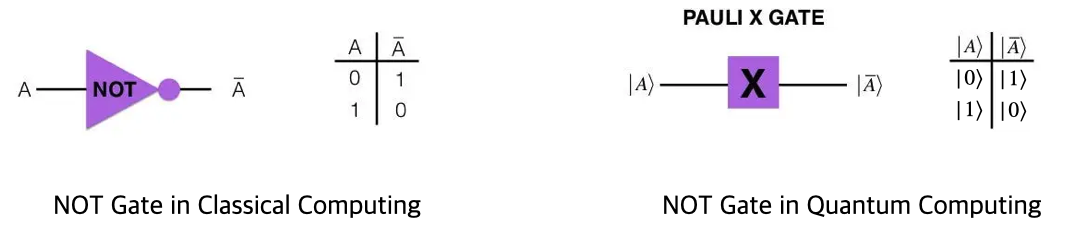
\includegraphics[width=0.8\linewidth]{figs/Not Gates.png}
    \caption{NOT Gates in Classical/Quantum Computing}
    \label{fig:NOT-Gates}
\end{figure}

고전 논리 회로에서 NOT 게이트는 [그림3.1]과 같이 input이 0인 경우 output으로 1을 내놓고, input이 1인 경우 output으로 0을 내놓는 역할을 한다. 이는 \(\mathbb{Z}_2\)에서 \( \text{NOT } A = A + 1\)과 같다.

양자 논리 회로에서 NOT Gate는 특별하게 Pauli-X Gate라고 불리며, [그림3.1]과 같이 input이 \(\ket 0\)인 경우 output으로 \(\ket 1\)을, input이 \(\ket 1\)인 경우 output으로 \(\ket 0\)을 내놓는 역할을 한다.

이 Operation은 다음과 같이 나타나는데:
\begin{align*}
    X\ket{0} &= \ket{1}  \\
    X\ket{1} &= \ket{0}
\end{align*}
따라서 \(X\)가 다음과 같은 matrix form을 가져야 함을 어렵지 않게 추론할 수 있다.
\[
    X = \begin{pmatrix}
        0 & 1 \\
        1 & 0
    \end{pmatrix}
\]
이와 같이, qubit state는 벡터이고, qubit에 가해지는 operation은 행렬로 나타난다.

\noindent 하지만 qubit state vector는 몇 가지 특별한 특징을 갖는다는 것을 알고 있다. 특히, qubit들은 normalize 되어야 한다. 즉, 길이가 1이다. 따라서 qubit에 작동하는 모든 matrix는 vector의 크기를 보존하는 구조를 필요로 한다. 선형대수학에서, 이러한 특징을 갖는 matrix를 Unitary Matrix라고 하며, Unitary Matrix는 다음과 같은 추가적인 필요충분조건을 갖는다.

\noindent \(\text{for } n \times n \text{ Unitary Matrix }U \text{, } {\sf TFAE} \)
\begin{flalign*}
    & \text{1. } U^\dagger = U^{-1} \\
    & \text{2. } UU^\dagger = U^\dagger U = I_n \\
    & \text{3. rows of } U \text{ are orthonormal} \\
    & \text{4. columns of } U \text{ are orthonormal} \\
    & \text{5. } {}^{\forall}\mathbf{x, y} \in \mathbb{C}^n, U\mathbf{x} \cdot U\mathbf{y} = \mathbf{x} \cdot \mathbf{y} \\
    & \text{6. } {}^{\forall}\mathbf{x} \in \mathbb{C}^n, || U\mathbf{x} || = || \mathbf{x} ||
\end{flalign*}
\noindent 가장 중요한 것은 1번째 성질로, \(U\)의 inverse \(U^{-1}\)는 \(U^\dagger\) 즉, \(U\)를 transpose하고, 모든 entry에 conjugate을 취한 것과 같다는 것이다.

\subsubsection{3.2.3.2 \quad Single Qubit Gates}
모든 qubit operation이 Unitary Matrix인 것과 같이, 모든 Unitary Matrix는 그 자체로 qubit operation이 된다. [표 3.1]과 같이 다양한 용도의 Unitary Operation이 존재한다:

\begin{table}[htb!]
    \centering
    \begin{tabular}{|c|c|c|c|c|}
        \hline
         Name & Symbol & Matrix & Basis state action \\ \hline

         Pauli-X & X & \(\begin{pmatrix} 0 & 1 \\ 1 & 0 \end{pmatrix}\) & \begin{tabular}[l]{@{}l@{}} $X\ket{0} = \ket{1}$\\ $X\ket{1} = \ket{0}$ \end{tabular} \\ \hline

         Pauli-Y & Y & \(\begin{pmatrix} 0 & -i \\ i & 0 \end{pmatrix}\) & \begin{tabular}[l]{@{}l@{}} $Y\ket{0} = i\ket{1}$\\ $Y\ket{1} = -i\ket{0}$ \end{tabular} \\ \hline

         Pauli-Z & Z & \(\begin{pmatrix} 1 & 0 \\ 0 & -1 \end{pmatrix}\) & \begin{tabular}[l]{@{}l@{}} $Z\ket{0} = \ket{0}$\\ $Z\ket{1} = -\ket{1}$ \end{tabular} \\ \hline

         Hadamard & H & \(\displaystyle {1\over\sqrt{2}}\begin{pmatrix} 1 & 1 \\ 1 & -1 \end{pmatrix}\) & \begin{tabular}[l]{@{}l@{}} $\displaystyle H\ket{0} = {1\over\sqrt{2}}\left(\ket{0} + \ket{1} \right) $ \\ $\displaystyle H\ket{1} = {1\over\sqrt{2}}\left(\ket{0} - \ket{1} \right) $ \end{tabular} \\ \hline

         S & S & \(\begin{pmatrix} 1 & 0 \\ 0 & i \end{pmatrix}\) & \begin{tabular}[l]{@{}l@{}} $S\ket{0} = \ket{0}$\\ $S\ket{1} = i\ket{1}$ \end{tabular} \\ \hline

         T & T & \(\begin{pmatrix} 1 & 0 \\ 0 & {e^{i\pi / 4}} \end{pmatrix}\) & \begin{tabular}[l]{@{}l@{}} $T\ket{0} = \ket{0}$\\ $T\ket{1} = e^{i\pi / 4}\ket{1}$ \end{tabular} \\ \hline

         $RX$ & $RX$ & \(\displaystyle \begin{pmatrix} \cos\left({\theta \over 2}\right) & -i\cdot\sin\left({\theta \over 2}\right) \\ -i\cdot\sin\left({\theta \over 2}\right) & \cos\left({\theta \over 2}\right) \end{pmatrix}\) & \begin{tabular}[l]{@{}l@{}} $\displaystyle RX(\theta) \ket{0} = \cos{\theta \over 2}\ket{0} -i\sin{\theta\over 2}\ket{1}$\\ $\displaystyle RX(\theta)\ket{1} = -i\sin{\theta \over 2}\ket{0} -\cos{\theta\over 2}\ket{1}$ \end{tabular} \\ \hline

         $RY$ & $RY$ & \(\displaystyle \begin{pmatrix} \cos\left({\theta \over 2}\right) & -\sin\left({\theta \over 2}\right) \\ \sin\left({\theta \over 2}\right) & \cos\left({\theta \over 2}\right) \end{pmatrix}\) & \begin{tabular}[l]{@{}l@{}} $\displaystyle RY(\theta) \ket{0} = \cos{\theta \over 2}\ket{0} + \sin{\theta\over 2}\ket{1}$\\ $\displaystyle RY(\theta)\ket{1} = -\sin{\theta \over 2}\ket{0} +\cos{\theta\over 2}\ket{1}$ \end{tabular} \\ \hline

         $RZ$ & $RZ$ & \(\displaystyle \begin{pmatrix} e^{-i{\theta \over 2}} & 0 \\ 0 & e^{i{\theta \over 2}} \end{pmatrix}\) & \begin{tabular}[l]{@{}l@{}} $\displaystyle RZ(\theta) \ket{0} = e^{-i{\theta \over 2}}\ket{0}$\\ $ RZ(\theta)\ket{1} = e^{i{\theta \over 2}}\ket{1}$ \end{tabular} \\ \hline
    \end{tabular}
    \caption{Single Qubit Gates : Matrix and Actions}
    \label{tab:single qubit gates}
\end{table}
[표 3.1]에 나타난 여러 Single Qubit Gate 중, Hadamard Gate는 \(\ket{0}\)에 적용했을 때 \(\ket 0\)과 \(\ket 1\)의 상태가 동일한 확률로 중첩되도록 하는 gate이다. 또한 RX, RY, RZ Gate의 동작을 이해하기 위해서는, 아래 식과 같이 single qubit state를 매개변수화하고, 이를 [그림 3.2]의 Bloch Sphere를 통해 시각화하면 그 동작이 직관적으로 이해된다:
% 또한 RX, RY, RZ Gate의 경우 다음과 같이 매개변수화된 single qubit state와, 이를 시각화한 Bloch Sphere를 통해 그 동작이 직관적으로 이해된다:
\[
    \ket{\psi(\theta, \phi)} = \cos{\left({\theta \over 2}\right)}\ket 0 + \sin{\left({\theta \over 2}\right)}e^{i\phi} \ket 1
\]
% \textit{global phase를 배제한 }
위와 같이 single qubit state를 변수 \(\theta, \phi\)에 대해 매개변수화하면, 구면좌표로 표현된 3차원 공간에서, qubit state와 unit vector간의 연관성을 만들 수 있다. 이 연관성을 통해 single qubit에서의 state 및 operation의 구조와 동작을 이해하는 시각화 도구인 Bloch Sphere([그림 3.2])가 고안되었다.
\begin{figure}[htb!]
    \centering
    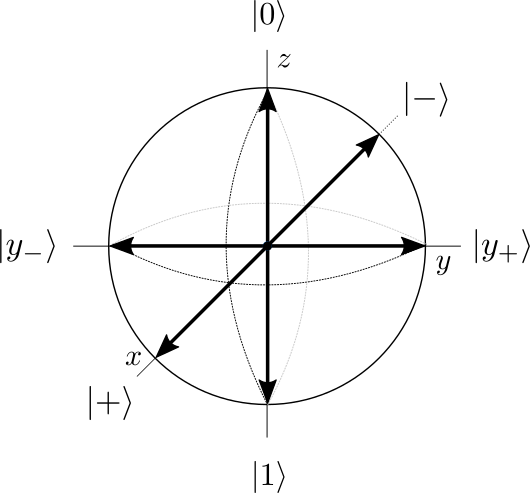
\includegraphics[width=0.5\linewidth]{figs/bloch_sphere.png}
    \caption{Bloch Sphere}
    \label{fig:bloch-sphere}
\end{figure}

\noindent Bloch Sphere에는 세 개의 축($x, y, z$)이 있다. z축에서, 맨 위의 상태는 $|0\rangle$, 맨 아래의 상태는 $|1\rangle$을 의미한다. 이는 Pauli Z operator의 eigenvector들이다. 유사하게, x축에는 $|+\rangle = {1\over \sqrt 2}\left(|0\rangle + |1\rangle\right)$, $|-\rangle = {1\over \sqrt 2}\left(|0\rangle - |1\rangle\right)$ 상태가 있고, 이는 Pauli X operator의 eigenvector들이다. y축에 대해서도 비슷한 결과를 얻을 수 있다.
\begin{figure}[htb!]
    \centering
    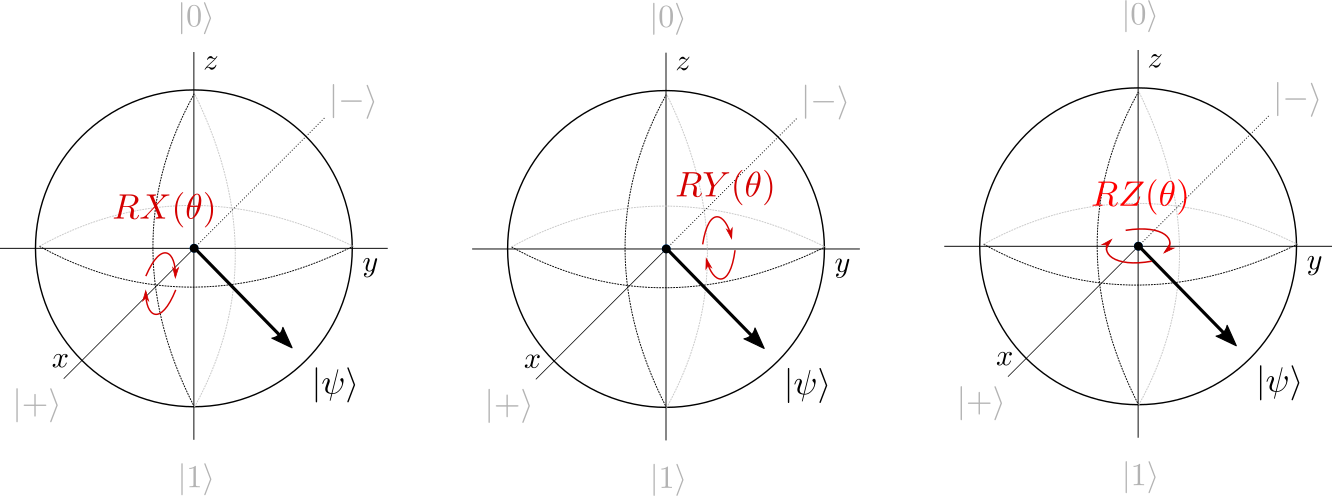
\includegraphics[width=1.0\linewidth]{figs/RXRYRZ.png}
    \caption{RX, RY, and RZ operations on Bloch Sphere}
    \label{fig:RX RY RZ}
\end{figure}

[그림 3.3]을 통해, RX, RY, RZ Gate의 동작에 대해 시각적으로 이해할 수 있다. Bloch Sphere 위의 한 점은 single qubit state 하나에 대응되고, RX, RY, RZ Gate는 주어진 매개변수 \(\theta\)만큼, 각 축에 대해 반시계방향으로 회전하는 것과 같다.

\subsubsection{3.2.3.3 \quad Universal Gate Set}
고전 논리 게이트에서, 모든 논리 게이트를 \(\{AND, OR, NOT\}\)의 조합으로 구성할 수 있으며 이를 Universal Gate Set이라고 한다. 양자 게이트도 마찬가지로 Universal Gate Set이 존재하는데, 모든 single qubit operation, 즉 모든 unitary를 구성하기 위해서는 [표 3.1] 중 \(\{RX, RY\}\), \(\{RY, RZ\}\), \(\{RZ, RX\}\)와 같이 \(\{RX, RY, RZ\}\) 중 2개의 operation을 선택하면, 그들의 조합만으로 모든 Unitary를 구성할 수 있다. 예컨대 \(\{RY, RZ\}\)만으로 모든 Unitary를 구성할 수 있음을 살펴보자.

\noindent 먼저, 모든 Unitary Matrix는 다음과 같이 3개의 매개변수 \(\phi, \theta, \omega\)로 표현이 가능하다.
\[
U(\phi, \theta, \omega) = \left( \begin{matrix}
 e^{-i(\phi + \omega)/2}\cos(\theta/2) & {-e^{i(\phi - \omega)/2}\sin(\theta/2) }
\\
 e^{-i(\phi - \omega)/2}\sin(\theta/2) & {e^{i(\phi + \omega)/2}\cos(\theta/2) }
\end{matrix}
\right)
\]

\noindent 이는 다음과 같이, \(RZ, RY\)으로 decompose될 수 있다.

\begin{align*}
    RZ(\omega)RY(\theta)RZ(\phi) &= \begin{pmatrix} e^{-i{\omega \over 2}} & 0 \\ 0 & e^{i{\omega \over 2}} \end{pmatrix} \begin{pmatrix} \cos\left({\theta \over 2}\right) & -\sin\left({\theta \over 2}\right) \\ \sin\left({\theta \over 2}\right) & \cos\left({\theta \over 2}\right) \end{pmatrix} \begin{pmatrix} e^{-i{\phi \over 2}} & 0 \\ 0 & e^{i{\phi \over 2}} \end{pmatrix} \\
    &= \begin{pmatrix} e^{-i{\omega \over 2}}\cos\left({\theta \over 2}\right) & -e^{-i{\omega \over 2}}\sin\left({\theta \over 2}\right) \\ e^{i{\omega \over 2}}\sin\left({\theta \over 2}\right) & e^{i{\omega \over 2}}\cos\left({\theta \over 2}\right) \end{pmatrix} \begin{pmatrix} e^{-i{\phi \over 2}} & 0 \\ 0 & e^{i{\phi \over 2}} \end{pmatrix} \\
    &= \begin{pmatrix}
     e^{-i(\phi + \omega)/2}\cos(\theta/2) & {-e^{i(\phi - \omega)/2}\sin(\theta/2) } \\
     e^{-i(\phi - \omega)/2}\sin(\theta/2) & {e^{i(\phi + \omega)/2}\cos(\theta/2) }
    \end{pmatrix} \\
    &= U(\phi, \theta, \omega) \quad \square
\end{align*}

이처럼 single qubit gate의 Universal Gate Set이 존재하고, 이는 양자 머신러닝의 General한 모델을 구성하는데 중요한 역할을 한다.

% --> Thm으로 쓰고 Proof를 넣을까? Proof 자체는 들어가긴 해야할 듯 Reference를 달던지

% 현재 시간 12월 3일 오전 2시 56분... 내일부턴 Universal Gate Set과(고민해보고) Multi-qubit gate 설명해야 함..

\subsubsection{3.2.3.4 \quad Multi Qubit Gate}
% 여러 qubit에 대한 연산은 두 가지 형태로 표현이 가능하다. 첫 번째 형태는 근본적으로 개별(individual) 큐비트에 대한 단일 큐비트 연산을 수행하는 것처럼 보이지만, 다중 큐비트 시스템에서는 여러 single qubit 연산을 병렬로 적용할 수 있다. 단순히 개별 큐비트 연산의 텐서 곱으로 표현될 수 있기 때문에 이를 분리 가능한 연산(seperable operation)이라고 부른다.

여러 qubit에 대한 연산은, qubit의 개수에 따라 그 크기에 맞는 Unitary Matrix로 이루어진다. 예컨대 2 qubit state의 경우 normalize된 4-dimension complex vector이고, 따라서 Quantum Gate로 \(4 \times 4\) Unitary Matrix를 사용한다. 이를 일반화하면, $n$ qubit state에 대한 Operation은 \(2^n \times 2^n\) Unitary Matrix를 사용함을 알 수 있다.

이러한 multi-qubit gate를 두 가지 종류로 분류할 수 있다. 첫 번째는 각각의 qubit에 독립적으로 single-qubit gate가 가해지는 것이고, 두 번째는 여러 qubit이 결부되어 operation이 가해지는 것이다.

\noindent 먼저 첫 번째 예시를 살펴보기 전에, 두 Matrix간의 tensor product를 정의한다.
\begin{definition}
Tensor product \(\otimes\) between Matrix

Let \( A \) and \( B \) be \(2 \times 2\) matrices defined as:
\[
A = \begin{pmatrix}
a_{11} & a_{12} \\
a_{21} & a_{22}
\end{pmatrix}, \quad
B = \begin{pmatrix}
b_{11} & b_{12} \\
b_{21} & b_{22}
\end{pmatrix}.
\]

The \textbf{tensor product} \( A \otimes B \) is defined as:
\[
A \otimes B =
\begin{pmatrix}
a_{11}B & a_{12}B \\
a_{21}B & a_{22}B
\end{pmatrix},
\]
where each entry \( a_{ij}B \) is a scalar multiple of the matrix \( B \).

Explicitly, we have:
\[
A \otimes B =
\begin{pmatrix}
a_{11}b_{11} & a_{11}b_{12} & a_{12}b_{11} & a_{12}b_{12} \\
a_{11}b_{21} & a_{11}b_{22} & a_{12}b_{21} & a_{12}b_{22} \\
a_{21}b_{11} & a_{21}b_{12} & a_{22}b_{11} & a_{22}b_{12} \\
a_{21}b_{21} & a_{21}b_{22} & a_{22}b_{21} & a_{22}b_{22}
\end{pmatrix}
\]

Likewise, for arbitrary matrices A(\(n_A \times m_A\)) and B(\(n_B \times m_B\)), tensor product \( A \otimes B \) is defined as:
\[
A \otimes B =
\begin{pmatrix}
a_{11}B & a_{12}B & \cdots & a_{1m_A}B \\
\vdots &          & \ddots & \vdots  \\
a_{n_A 1}B & a_{n_A 2}B & \cdots & a_{n_A m_A}B
\end{pmatrix}
\]
\end{definition}

\noindent 이제, 각 qubit에 독립적으로 가해지는 multi-qubit operation의 예시를 살펴보자.

\begin{example} % 당연하다는 듯이 써도 되나? 주의
multi-qubit gate as product of single-qubit gates

\noindent \(\ket{00} = \ket{0} \otimes \ket{0}\)과 같은 2 qubit state가 있다고 생각하자. 이때 첫 번째 qubit에 \(U_1\) gate, 두 번째 qubit에 \(U_2\) gate를 적용함을 생각하면, 다음과 같이 기술할 수 있다.

\[
\ket{00} \xrightarrow[]{U_1 \text{ for 1st qubit, } U_2 \text{ for 2nd qubit}} U_1\ket{0} \otimes U_2\ket{0}
\]

\noindent 이는 수학적으로 \((U_1 \otimes U_2)\ket{00}\)과 동일하며, 일반적인 multi-qubit gate에 대하여 성립한다.
\end{example}

다음으로, 여러 qubit이 결부된 multi-qubit gate의 예시로, CNOT(Controlled-NOT) gate를 살펴보자.
\begin{example}
CNOT gate as entangling gate

\[CNOT = \begin{pmatrix}
    1 & 0 & 0 & 0 \\
    0 & 1 & 0 & 0 \\
    0 & 0 & 0 & 1 \\
    0 & 0 & 1 & 0 \\
\end{pmatrix}\]

\noindent 위 행렬로 나타나는 CNOT gate는 다음 진리표([표 3.2])와 같이 작동하는데:

\begin{table}[htb!]
    \centering
    \begin{tabular}{|c|c|c|c|c|}
        \hline
         Input & Output \\ \hline
         $\ket{00}$ & $\ket{00}$ \\ \hline
         $\ket{01}$ & $\ket{01}$ \\ \hline
         $\ket{10}$ & $\ket{11}$ \\ \hline
         $\ket{11}$ & $\ket{10}$ \\ \hline
    \end{tabular}
    \caption{Operation of CNOT Gate}
    \label{tab:CNOT Operation}
\end{table}
진리표를 통해, 첫 번째 qubit(control bit라고 한다)의 state가 $\ket 1$이면 두 번째 qubit(target bit라고 한다)에 Pauli-X gate(NOT gate)를 동작시킨다는 것을 확인할 수 있다. 만약 control bit의 state가 $\ket 0$인 경우 아무런 동작도 하지 않는다.
\noindent $CNOT$ gate와 같이, 두 single-qubit unitary의 tensor product로 나타나지 않는 gate는 다양한 경우에 두 qubit 사이의 관계를 형성하게 되어 \textbf{entangling gate}라고 한다.
\end{example}

\noindent 또한 다음과 같이 일반적인 two-qubit Controlled-Unitary를 구성할 수 있다.

% \text{for } $U \in U(n)$,
\(\text{for } 2 \times 2 \text{ Unitary Matrix }U \text{,}\)

\[
    CU = \begin{pmatrix}
        I_2 & O \\
        O & U \\
    \end{pmatrix}
\]

위와 같이 정의된 two-qubit gate $CU$는, control bit인 첫 번째 qubit의 state가 $\ket 0$인 경우 아무런 동작도 하지 않고, control bit의 state가 $\ket 1$인 경우 target bit인 두 번째 qubit에 single-qubit gate $U$를 동작시킨다. 앞서 살펴본 $CNOT$ gate의 경우 위와 같이 일반적으로 정의된 $CU$에서 $U$에 Pauli-X를 대입한 것과 같다.

\noindent Quantum gate를 이해하기 위해, 마지막으로 다음 예시를 살펴보자.
\begin{example}
    Algorithm to make Bell State

먼저 two-qubit state \(\ket{00}\)를 준비하고, 다음 Step을 밟는다.
\begin{flalign*}
    & \text{1. 첫 번째 qubit에 Hadamard gate를 취한다.}  \\
    & \text{2. 첫 번째 qubit을 control bit, 두 번째 qubit을 target bit로 하는 CNOT gate를 취한다.}
\end{flalign*}
Step 1의 결과는 다음과 같다.
% \[
%     \ket{00} \xrightarrow[]{H \text{ for 1st qubit}} H\ket{0} \otimes \ket{0} = \left({\ket{0} + \ket{1} \over \sqrt{2}}\right) \otimes \ket{0}
% \]
\begin{flalign*}
    \ket{00} \xrightarrow[]{H \text{ for 1st qubit}} H\ket{0} \otimes \ket{0} &= \left({\ket{0} + \ket{1} \over \sqrt{2}}\right) \otimes \ket{0} \\
    &= {1\over \sqrt{2}}\left(\ket{00} + \ket{10}\right)
\end{flalign*}
즉, 첫 번째 qubit에는 $\ket 0$과 $\ket 1$이 동일한 확률로 중첩되어 있고, 두 번째 qubit은 원상태($\ket 0$)를 유지한다.

\noindent 다음으로, Step 2의 연산을 수행하면:
\[
    {CNOT}  \left({\ket{00} + \ket{10} \over \sqrt{2}} \right) = {\ket{00} + \ket{11} \over \sqrt{2}}
\]
즉, Step 1과 Step 2의 연산 결과 1번째 qubit의 state가 $\ket 0$이면 2번째 qubit의 state도 $\ket 0$이고, 1번째 qubit의 state가 $\ket 1$이면 2번째 qubit의 state도 $\ket 1$인 가장 기본적인 entangled state를 생성하게 된다. 3.2.2장에서 살펴보았던, 이 state를 특별히 Bell State라고 한다.

\end{example}

\subsection{Quantum Circuit} % 마지막으로, 양자컴퓨팅의 개념 중 양자 회로에 대해 소개하고 이번 section을 마무리한다.
양자 회로(Quantum Circuit)는 양자 계산 중에 qubit에서 수행되는 일련의 작업들을 시각적으로 표현하는 일반적인 방법이다. 이들은 qubit(또는 wire라는 표현을 사용한다) 세트에 적용되는 연산 또는 게이트 세트로 구성된다. 양자 회로 다이어그램에서의 각 wire는 qubit을 나타낸다. 회로는 왼쪽에서 오른쪽으로 읽고, 이것은 operation이 적용되는 순서이다. 양자회로는 하나 이상의 큐비트의 측정(measurement)이 이루어지면 종료된다.

각 gate의 양자 회로 표현은 [그림 3.4]와 같다.
\begin{figure}[htb!]
    \centering
    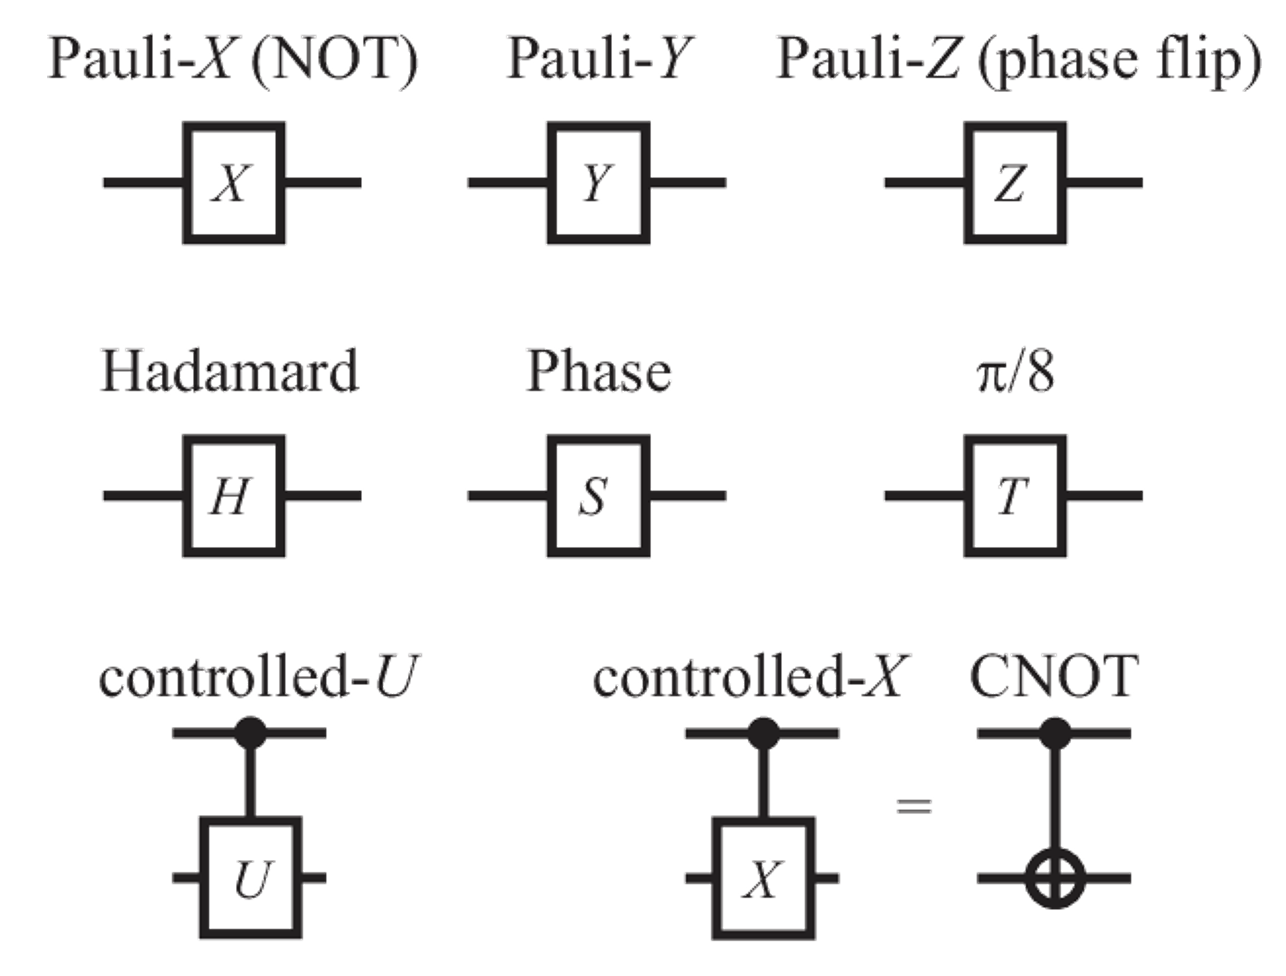
\includegraphics[width=0.45\linewidth]{figs/QuantumGateSymbols.png}
    \caption{Circuit representation of elementary quantum gates}
    \label{fig:quantum gate symbols}
\end{figure}

\begin{figure}[htb!]
    \centering
    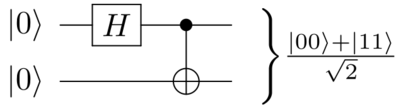
\includegraphics[width=0.5\linewidth]{figs/BellStateCircuit.png}
    \caption{Bell State Preparation Circuit}
    \label{fig:bell state circuit}
\end{figure}

[그림 3.5]는 Example 3.2.3에서의 연산과정을 양자회로로 표현한 것으로, 첫 번째 qubit에 Hadamard gate를, 이후 CNOT gate를 가동한 과정을 행렬식이나 bra-ket notation으로 표현한 것보다 직관적으로 이해할 수 있다.

양자 회로는 곧 양자 알고리즘이다. 보편적인 프로그래밍에서 알고리즘과 소프트웨어의 복잡도(complexity) 및 resource requirement를 고려하여 그 효율성을 높이는 것처럼, 양자 회로에 대해서도 동일한 과제가 주어진다. 양자 회로의 효율성을 평가하는 한 가지 중요한 기준은 바로 \textbf{Circuit Depth}이다. 여기서 Depth는, 가능한 한 병렬로 연산이 수행될 경우 회로가 작동하는 데 걸리는 시간 단계를 의미한다. 또는 회로의 layer 수라고 생각할 수 있다. 예컨대, [그림 3.5]에 나타난 회로의 경우 2의 depth를 가진다.

\subsection{Measurement and Expectation Value}
지금까지 quantum computer의 연산이 어떻게 동작되는지에 대해서 살펴보았다. 하지만 실제 문제를 해결하려고 하면, 일련의 알고리즘을 수행한 이후의 qubit state를 해석하여서 직면한 문제와 다시 연관시킬 수 있는 방법이 필요하다. 이에 전술한 것과 같이, 모든 양자 알고리즘은 다양한 방식으로의 병렬 연산을 수행한 후, 마지막으로 정보를 추출하기 위한 최종 단계를 거친다. 이때 마지막 정보 추출의 과정에 사용되는 연산은 Unitary 연산은 아니다. 따라서, 양자 알고리즘의 최종 단계인 Measurement와 Expectation Value에 대해 살펴보고 3.2장을 마친다.

\subsubsection{3.2.5.1 \quad Measurement}
다음과 같은 qubit state를 가정하자.
$$
|\psi \rangle = \alpha |0\rangle + \beta |1\rangle
$$
먼저, 이전에 살펴본 것은 위 qubit을 측정하면, $|0\rangle$으로 측정될 확률은 $|\alpha | ^2 = \alpha\alpha^*$이고, $|1\rangle$으로 측정될 확률은 $|\beta|^2$라는 것이다. measurement outcome probability를 표현하는 조금 더 formal한 방법은, inner product를 사용하는 것이다. quantum state $|\psi\rangle$가 주어지면, 그 state가 $|\phi \rangle$ state로 측정될 확률 \(\Pr(\phi)\)은 다음과 같다.% (basis that includes $|\phi \rangle$)
\begin{definition}
    probability that state \(\ket\psi\) is measured by state \(\ket\phi\)
$$
\Pr(\phi) = |\langle \phi |\psi \rangle | ^2
$$
\end{definition}
다음 예시를 살펴보자:
\begin{example}
    computing $\Pr(0)$ and $\Pr(1)$ for $|\psi\rangle = \alpha|0\rangle + \beta|1\rangle$
\[
\Pr(0) = |\langle0|\psi\rangle|^2 =|\langle0|(\alpha|0\rangle +\beta|1\rangle)|^2 = |\alpha \langle0|0\rangle + \beta \langle0|1\rangle|^2 = |\alpha|^2, \\
\]
\[
\Pr(1) = |\langle1|\psi\rangle|^2 =|\langle1|(\alpha|0\rangle +\beta|1\rangle)|^2 = |\alpha \langle1|0\rangle + \beta \langle1|1\rangle|^2 = |\beta|^2
\]
\end{example}
이때, 사용되는 measurement 방식을 특별히 projective measurement라고도 한다. 기본적으로, “각 basis state가 주어진 state에 얼마나 기여하는가?”를 묻고 있는 것이다. 이 이름은 두 state vector의 inner product 즉, 선형대수에서의 projection과 같은 연산을 수행하고 있다는 사실에서 기인한다. 그러나 standard linear algebra와 다른 한 가지 단계는, 실제 확률 값을 얻기 위해서는 inner product의 제곱을 취해야 한다는 것이다.

\subsubsection{3.2.5.2 \quad Expectation Value}

측정 결과로 확률 정보를 얻는 것은 qubit의 state에 따라 유용한 정보를 제공하지만, 종종은 그 state가 갖는 에너지와 같은 물리적인 것에 관심이 있을 때가 있다. 양자역학에는 에너지(energy), 운동량(momentum), 위치(position) 등 Observable이라는 이름의 "관측 가능한" 특성을 가지는 물리량이 존재한다. 이는 수학적으로, 임의의 양자 상태에 대해 Observable Operator의 기댓값(Expectation Value)이 실수값이라는 의미인데, 이는 다음과 같이 계산된다.
\begin{definition}
    Expectation Value of Observable \(A\) in the state \(\ket \psi\)
    \[
        \bra{\psi}A\ket{\psi}
    \]
\end{definition}

위 정의와 같이 주어진 Observable \(A\)에 대한 expectation value가 계산되는데, 이때 얻게 되는 값은 행렬 A의 eigenvalue와 각각의 확률에 대한 linear comination으로 나타난다. 따라서 Observable의 expectation value로 실수값만을 얻게 된다는 것은 Observable Matrix가 real eigenvalue만을 갖는다는 것이고, 이는 선형대수에서의 Hermitian matrix(\(A^\dagger = A\))에 해당한다.

\noindent 다음 예시를 살펴보자:

\begin{example} Calculating Expectation Value for given Observable

\[
    \text{For } |\psi\rangle = {4\over 5}|0\rangle - {3 \over 5}e^{i\pi / 3}|1\rangle,
\]
\[
\text{ suppose we want to measure the obsevable } B = \left( \begin{matrix}
    1 & -2i \\
    2i & 2
    \end{matrix}\right)
\]

\begin{align*}
    % & \text{i) eigenvalues of } B : \lambda_1 = 3.56155281 , \lambda_2 = -0.56155281 \\
    % & \text{ii) }
    \text{Expectation Value of } B : \langle\psi|B|\psi\rangle = {1 \over 25} \left(\begin{matrix}4 & -3e^{i\pi/3}\end{matrix}\right)\left(\begin{matrix}
        1 & -2i \\
        2i & 2
        \end{matrix}\right)\left(\begin{matrix} 4 \\ -3e^{i\pi /3}\end{matrix}\right) = -0.302769
\end{align*}

\end{example}
위 예시로 알아볼 수 있듯, 문제에 맞게 미리 구성한 Observable(Hermitian Matrix)를 이용하여, 보유한 quantum state에서 적절한 실수값을 추출할 수 있다. 이는 양자 머신러닝의 마지막 부분으로서 중요한 역할을 한다.

% \section{Methods for Quantum Machine Learning}
% 설명(삭제예정) : 양자 머신러닝의 두 가지 방법론(PQC, Q-Perceptron)을 기술하는 장이다. (sin fitting 실험 기술 등), 또한 다양한 Data Encoding 방식, 측정(expval)을 통한 확률(정보) 추출 등\\
% 흠 근데 Q-Perceptron에 대한 설명은 다음 챕처에서 해야 하는데 여기서 실험을 언급하는 게 맞나 싶네



%#########################################################
%
% Author : SEHYUN YUK
% Last Update: 2024.12.08
%
%##########################################################



%#########################################################
% 3.3 Quantum Machine Learning
%
% Author : SEHYUN YUK
% Last Update: 2024.12.08
%
%##########################################################
\section{Quantum Machine Learning}

 이 장에서는 우리의 본래 목적인, QRF에서 사용된 QML의 세부 요소를 설명한다. 또한 두 가지 문제에 대해 ML과 QML 모델을 각각 구현하여 실제 ML과 QML의 결과값을 비교 분석해보고자 한다. 이를 위해 용어에 대한 정의와 개념을 명확히 하고, 이후 분석 내용과 결과를 서술한다.
 \subsection{Concepts} \label{qml:concepts}

 앞으로 사용하게 될 주요한 용어와 정의에 대해서 설명할 것이다.

\subsubsection{Classical Machine learning} 1950년대, Arthur Samuel은 머신러닝을 "명시적으로 프로그래밍되지 않고 컴퓨터가 학습할 수 있는 능력을 부여하는 연구 분야"로 정의하였다\citep{schuld2015introduction}. 즉, 머신러닝은 입력과 출력에 대한 관계를 데이터를 통해 발견해내는 알고리즘이라고 볼 수 있다. 이러한 머신러닝 중 \textbf{nerual network} 와 \textbf{back propagation}를 통해 학습하는 방법을 \textbf{deep learning}이라고 부른다.

nerual network 중 대표적으로 언급되는 것은 \textbf{mutil layer perceptron} 이라는 모델이다. 이 모델은 연결된 뉴런 또는 노드의 시스템으로 구성된다.\cite{gardner1998artificial} 여기서 하나의 노드는 수학적 함수로 표현이 가능한 모델이다. 이 모델의 출력은 가중치 $\mathbf{w} \in \mathbb{R}^n $와의 입력벡터 $\mathbf{x} \in \mathbb{R}^n $ 내적과 편향 $b \in \mathbb{R}$의 덧셈이 활성화함수 혹은 비선형함수라고 불리는 함수에 통과하게 되어 형성된다.\cite{krenker2011introduction}
이를 표현한 그래프를 보면 쉽게 이해할 수 있다. % 모델, 모델 ... -> 모델의 출력 대신 노드의 출력?이 맞지 않을까 일단 보류

\begin{figure}[htb!]
    \centering
    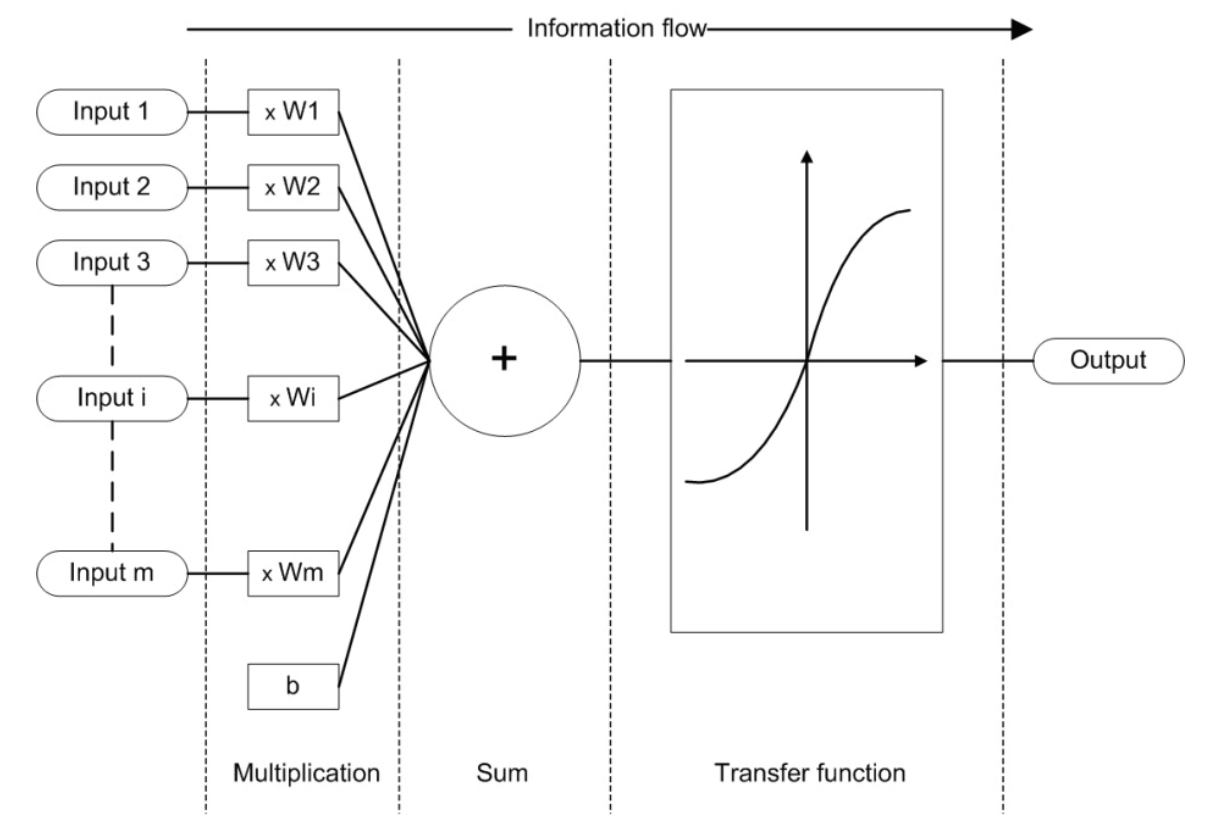
\includegraphics[width=0.8\textwidth]{figs/node.png}\
    \caption{Perceptron Architecture}
    \label{fig:node-image}
\end{figure}

이러한 노드들이 모이면 하나의 layer를 형성한다. 이렇게 형성된 layer 중 입력과 직접적으로 가중치 곱을 수행하는 layer를 \textbf{input layer}라고 하며, 최종적으로 노드의 출력이 마지막이 되는 layer를 \textbf{output layer}라고 한다. 그리고 input layer와 output layer 사이에 있는 layer들을 \textbf{hidden layer}라고 부른다.\cite{popescu2009multilayer} 이렇게 형성된 layer는 이전 layer의 노드들과 다음 layer의 노드들 간의 가중치 곱을 통해 연결되며, 이러한 가중치들은 이전 layer의 노드 개수 $N$, 다음 layer의 노드 개수 $M$ 과 함께 $N \times M $ 행렬로 표현된다. 이러한 가중치들은 bias와 함께 Backpropagation을 통해 학습 가능하기 때문에 \textbf{학습 파라미터}라고 불린다.

이렇게 형성된 multi perceptron layer는 다양한 비선형 함수를 근사할 수 있다는 장점과, 병렬연산이 가능한 행렬연산을 통한 빠른 추론, 입력데이터와 출력데이터를 범용적으로 선택할 수 있다는 장점 덕분에 많은 관심을 받았다.

\subsubsection{Components of Quantum Machine Learning}
quantum machine learning 분야는 지난 몇 년 동안 classical machine learning의 모델, 데이터 인코딩, 통계학적 방법등을 양자 알고리즘 및 양자정보이론을 통해 속도와 성능을 높이려는 노력과 함께 탄생하였다. 따라서 quantum machine learning은 입력 데이터와 출력 데이터의 관계를 찾아내어 가중치 혹은 파라미터를 학습시키는 양자 정보 처리 방법 중 하나라고 볼 수 있다.\cite{schuld2015introduction}. 여기서 나타나는 입력 데이터는 양자 정보 이론을 사용하기 위해 양자 컴퓨터가 처리 가능한 데이터로 변환하는 과정이 반드시 수행되어야 한다. 그러나 이를 수행하는 과정을 "input problem"이라고 할 만큼 계산량이 많기 때문에 중요한 과정이며 이를 개선하기 위한 연구들이 많이 진행되어왔다.\cite{biamonte2017quantum}

전술하였듯 양자컴퓨터가 처리가능한 데이터를 양자 데이터라고 부르는데, 이는 qubit들을 통해 처리 가능한 정보를 의미하며 양자상태, 양자 레지스터, 양자회로 등으로 다양하게 나타날 수 있다.이렇게 기존에 보유한 데이터를 양자 데이터로 전환하는 과정을 \textbf{qunatum encoding}이라고 하는데 encoding 방식에 따라 \textbf{angle encoding}, \textbf{basis encoding}, \textbf{amplitude encoding}으로 불리우며, quantum autoencoder와 같이 새로운 방식들이 등장하고 있다.\cite{rath2023quantum}

\textbf{basis encoding}은 이러한 encoding 방식 중 가장 간단한 방식이다. 이 방법은 고전 데이터를 그대로 qubit state의 텐서곱으로 표현하는 것이다. 예를 들어 고전 데이터 5(101)가 주어진다면, 이를 다음과 같은 방법으로 매핑된다고 볼 수 있다.
\[
5 \mapsto |101\rangle = |1\rangle \otimes |0\rangle \otimes |1\rangle
\]
이는 정수형이나 문자열 등 주로 이산적인 데이터를 다룰때 사용하는 방식이다.

\textbf{Angle Encoding}은 입력 데이터를 qubit state의 phase에 encoding하는 방식으로, qubit circuit을 통해 이를 효율적으로 다룰 수 있기 때문에 중요한 방법이다. 또한 이를 활용하여 파라미터를 circuit안에 넣어 학습시킬 수 있는 parameter quantum circuit에 사용되기 때문에 더욱 중요하다. angle encoding은 RX, RY, RZ와 같은 rotation gate를 통해 하나의 qubit에 하나의 angle $\theta$ 값을 encoding한다. 예컨대 single qubit gate에 RX gate를 통해 angle encoding된 state는 다음과 같이 나타난다. % PQC는 삭제 요망

\[
|\psi(\theta)\rangle = R_y(\theta)|0\rangle + e^{i\phi}R_y(\theta)|1\rangle
\]
여기서 $e^{i\phi}$는 phase factor라고 불리우는 amplitude이며, 여기에 있는 $\phi$는 경우에 따라 사용되거나 무시될수 있다. 이를 qubit이 $n$개, 입력데이터 $\theta$가 n개 주어졌을때를 일반화하면 다음과 같이 표현된다.
\[
        |\psi(\theta_1, \ldots, \theta_n)\rangle = \bigotimes_{i=1}^n (R_y(\theta_i)|0\rangle + e^{i\phi_i}R_y(\theta_i)|1\rangle)
\]

% \clearpage
\textbf{Amplitude Encoding}은 데이터를 quantum state의 amplitude에 Encoding하는 방법이다. 이러한 방법은 n개의 qubit으로 $N := 2^n$개의 basis state coefficients에 데이터를 최대 $N$개 encoding 한다. 이를 일반화하여 표현하면 다음과 같다\cite{maronese2022quantum}

\[
|\psi_x\rangle = \sum_{i=0}^{N-1} \frac{x_{i}}{\norm{x}} |i\rangle
\]
여기서 입력 데이터 $\mathbf{x}$는 보통 N차원의 벡터가 된다. 이러한 encoding 방식은 기하 급수적인 qubit 효율 덕분에, 많은 양의 데이터를 압축해서 사용할 수 있지만, complex amplitude들을 encoding 할 경우 n개의 qubit을 사용할때 $\mathcal{O}(2^n)$의 depth가 요구된다는 단점이 있다.\cite{mitsuda2024approximate}

\textbf{Parameterized Quantum Circuit(PQC)}는 이렇게 encoding된 quantum data를 문제에 맞는 output state로 변환하는 역할을 하는 양자 회로이다. PQC는 고전적인 머신러닝 모델과 유사한 방식으로 작동하며, 최적의 결과를 도출하기 위해 양자 회로의 매개변수가 조정된다.이를 n개의 qubit이 주어졌을 때를 일반화하면 다음과 같이 표현될 수 있다.
\[
|\psi\rangle = \prod_{\ell=1}^{m} W_{\ell} u_{\ell}(\theta_{\ell}) |\psi_0\rangle
\]
여기서 \( |\psi_0\rangle \)는 초기 양자 상태를 나타내며, \( m \)은 layer의 반복 횟수, \( W_{\ell} \)는 \(\ell\)-번째 레이어에서의 비매개변수화된 양자 게이트, \( U_{\ell}(\theta_{\ell}) \)는 매개변수 \(\{\theta_0, \theta_1, \ldots, \theta_k\}\)를 가지는 \(\ell\)-번째 레이어에서의 매개변수화된 양자 게이트를 나타낸다. 이러한 pqc 회로는 data encoding 과정을 제외하면, mlp와 동일한 구조이지만 더 적은 파라미터와의 연산을 통해 출력이 나오는 구조이기 때문에, mlp를 대체하여 성능을 높이려는 방식으로 연구가 진행되고 있다. 이러한 연구중 하나가 우리에게 동기를 주었던 QRF이며 해당 연구에서 실제로 mlp를 pqc를 전환하였을때, 속도와 성능의 개선되었다는 것을 실험으로 보였다.\cite{yang2022quantum}
% 이때, \( u_{\ell}(\theta_{\ell}) \)의 형태는 물리적 제약(예: 물리적 큐비트 간의 연결성 제한)에 따라 달라질 수 있다. 생략

%#########################################################
% 3.3.2 Components of QML
%
% Author : SEHYUN YUK
% Last Update: 2024.12.08
%
%##########################################################
\subsection{Comparsion with QML and ML} \label{qml:comparision}

이 장은 우리의 본래 목적인 실험적으로 드러나는 QML과 ML의 차이를 수학적으로 보이는 장이다. 공평한 비교를 위해 똑같은 데이터를 사용하고, 똑같은 파라미터의 개수를 사용하였을 때, 특정함수를 추정하는 Task에서의 성능차이를 보이고자 하였다. 먼저 QRF논문에서 사용된 2d image를 reconstruction 하는 Task에서 작동방식을 확인하고, 이를 더 확실하게 검증하기 위해 1차원 함수를 추정하는 Task에서 또한 검증을 추가적으로 진행하였다.
\begin{itemize}
    \item \textbf{2d image reconstruction} :

        본 태스크는 xy 좌표를 입력으로 받아 RGB 값의 3차원을 예측하는 문제이다. 모델은 각 좌표 \((x, y)\)에 대해 색상 벡터 \((r, g, b)\)를 예측하며, 예측된 색상과 실제 색상 간의 손실을 계산하여 학습을 진행한다. 이를 수식으로 표현하면 다음과 같다.

            \[
            \text{Input}: \mathbf{p} = (x, y) \in \mathbb{R}^2
            \]

            \[
            \text{Prediction}: \hat{\mathbf{c}} = (\hat{r}, \hat{g}, \hat{b}) = f(\mathbf{p}; \theta)
            \]

            \[
            \text{Loss Function}: \mathcal{L}(\theta) = \frac{1}{N} \sum_{i=1}^{N} \| \hat{\mathbf{c}}_i - \mathbf{c}_i \|_2^2
            \]




            여기서 \(f\)는 모델 함수, \(\theta\)는 모델의 파라미터, \(N\)은 데이터 샘플의 수를 나타낸다. 모델은 손실 함수를 최소화하도록 파라미터 \(\theta\)를 최적화하여 예측된 RGB 값이 실제 값과 잘 일치하도록 학습된다. 여기서 ML과 QML의 차이는 모델과 데이터 인코딩에서만 차이나는데, 각각 다음과 같이 진행된다.


              \begin{table}[ht]
                    \centering
                    \begin{tabular}{ l||p{5.5cm}||p{5.5cm}}
                    \Xhline{3\arrayrulewidth}
                    \textbf{Item} & \textbf{MLP} & \textbf{QML} \\
                    \hline
                    Data Encoding & $(x,y) \in \mathbb{R}^2$을 $[-1 ,1]$ 사이로 정규화 하였다.    &
                    Angle Encoding을 사용하였다.$(x,y) \in \mathbb{R}^2$을 $[-1 ,1]$ 사이로 정규화한 이후 이 두 값을 3 개의 qubit 중 두개의 quibt에 RX gate에 $\theta_x ,\theta_y  $들을 각각 $ [-\pi ,\pi]$ 값 사이에 위치하도록 정규화하여  Angle encdoing 하였다.
                     \\
                    \hline
                    Model & MLP 모델을 사용하였으며, 입력에이어 1개 , 히든 레이어 1개 ,출력 레이어 1개로 구성하였으며, activation function은 RELU를 사용하였다. &
                    QRF에서 사용된 PQC 모델과 동일하도록 사용하였다. 총 3개의 qubit을 사용하였고, $ \prod_{0}^{2} RY_i(\theta)CX_i$ 의 gate를 3번 반복함으로써 3층의 레이어의 효과가 나타나도록 구현하였다. 이를 시각화면 다음과 같다.\labelcref{fig:2d-image}
                     \\
                    \Xhline{3\arrayrulewidth}
                    \end{tabular}
                    \caption{MLP와 QML의 비교}
                    \label{tab:mlp_qml_comparison}
                \end{table}

                % \clearpage
                \begin{figure}[h]
                    \centering
                    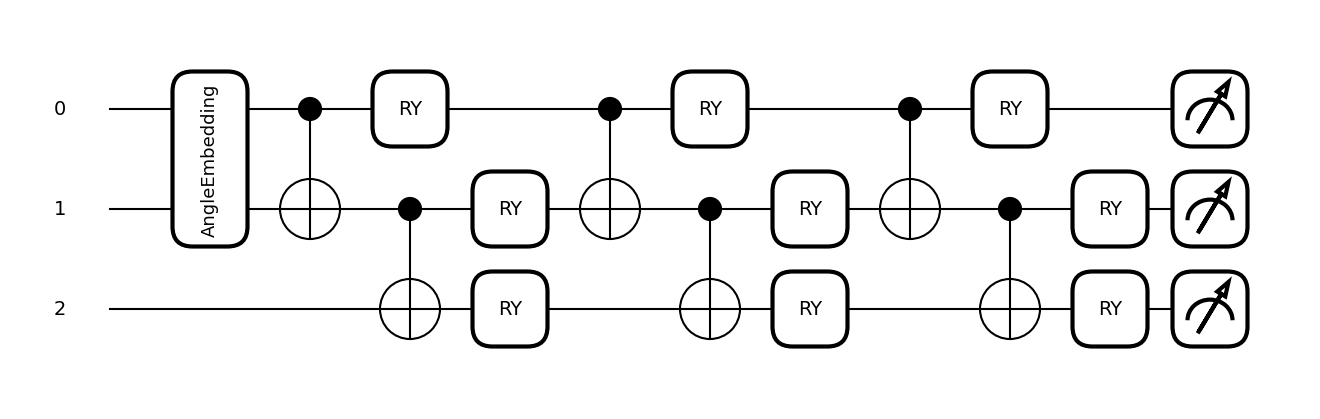
\includegraphics[width=0.8\textwidth]{figs/pqc_2d}\
                \caption{2-d image quantum circuit 구조}
                \label{fig:2d-image}
                \end{figure}

                이러한 모델은, 우리는 사진 3장(256x256)에 대하여, reconstruction error를 PSNR metric를 사용하여 학습된 성능을 평가하였다. PSNR의 수식은 다음과 같이 정의 된다.이는 높은 PSNR이 더 잘 reconstruction함을 뜻한다.

                \[
                    \text{PSNR} = 10 \cdot \log_{10}\left(\frac{\text{MAX}_I^2}{\text{MSE}}\right)
                    \]

                이와 같은 방법으로, 여러 layer별로 성능차이를 비교해보았으며, 결과는 다음과 같이 나타났다.

                \begin{table}[ht]
                    \centering
                    \begin{tabular}{c|ccc}
                    \Xhline{3\arrayrulewidth}
                    \multirow{2}{*}{Layers} & \multicolumn{3}{c}{PSNR (dB)} \\
                    \cline{2-4}
                    & Image 1 & Image 2 & Image 3 \\
                    \hline
                    MLP (3 layers) & 15.69 & 16.53 & 15.19 \\
                    MLP (4 layers) & 15.76 & 16.43 & 15.23 \\
                    MLP (5 layers) & 15.72 & 16.41 & 15.18 \\
                    \hline
                    PQC (3 layers) & 4.35 & 6.19 & 7.43 \\
                    PQC (4 layers) & 14.21 & 16.09 & 15.13 \\
                    PQC (5 layers) & 14.28 & 15.52 & 15.23 \\

                    \Xhline{3\arrayrulewidth}
                    \end{tabular}
                    \caption{PSNR comparison between MLP and QML models across different layer configurations}
                    \label{tab:psnr_comparison}
                \end{table}

        \item \textbf{1-d function estimation} :
본 태스크는 1차원 입력 x를 받아 스칼라 값 y를 예측하는 문제이다. 모델은 입력 x에 대해 출력 y를 예측하며, 예측된 값과 실제 값 간의 손실을 계산하여 학습을 진행한다. 이를 수식으로 표현하면 다음과 같다:

\[
\text{Input}: x \in \mathbb{R}
\]

\[
\text{Prediction}: \hat{y} = f(x; \theta)
\]

\[
\text{Loss Function}: \mathcal{L}(\theta) = \frac{1}{N} \sum_{i=1}^{N} (\hat{y}_i - y_i)^2
\]

여기서 \(f\)는 모델 함수, \(\theta\)는 모델의 파라미터, \(N\)은 데이터 샘플의 수를 나타낸다. 모델은 손실 함수를 최소화하도록 파라미터 \(\theta\)를 최적화하여 예측된 값이 실제 값과 잘 일치하도록 학습된다. ML과 QML의 차이는 모델과 데이터 인코딩에서만 차이나는데, 각각 다음과 같이 진행된다.


\begin{table}[ht]
    \centering
    \begin{tabular}{ l||p{5.5cm}||p{5.5cm}}
    \Xhline{3\arrayrulewidth}
    \textbf{Item} & \textbf{MLP} & \textbf{QML} \\
    \hline
    Data Encoding & $x \in \mathbb{R}$을 $[-1, 1]$ 사이로 정규화하였다. &
    Angle Encoding을 사용하였다. $x \in \mathbb{R}$을 $[-1, 1]$ 사이로 정규화한 이후, 이 값을 2개의 qubit 중 첫 번째 qubit의 RX gate에 $\theta_x$를 $[-\pi, \pi]$ 값 사이에 위치하도록 정규화하여 Angle encoding 하였다. \\
    \hline
    Model & MLP 모델을 사용하였으며, 입력 레이어 1개, 히든 레이어 2개, 출력 레이어 1개로 구성하였으며, activation function은 RELU를 사용하였다. &
    2개의 qubit을 사용하였고, $\prod_{0}^{1} RY_i(\theta)CX_i$의 gate를 3번 반복함으로써 3층의 레이어의 효과가 나타나도록 구현하였다.이를 다음과 같이 시각화하였다.\labelcref{fig:1d-image} \\
    \Xhline{3\arrayrulewidth}
    \end{tabular}
    \caption{MLP와 QML의 비교}
    \label{tab:mlp_qml_comparison_1d}
\end{table}

\begin{figure}[h]
    \centering
    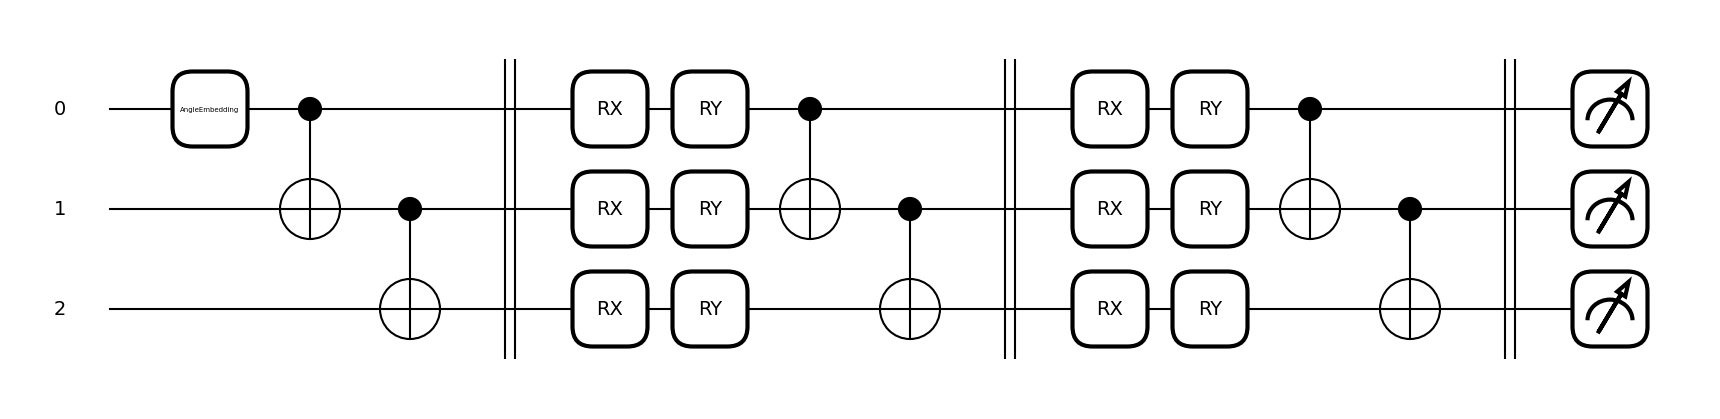
\includegraphics[width=0.8\textwidth]{figs/pqc_1d}\
\caption{1-d function estimation quantum circuit 구조}
\label{fig:1d-image}
\end{figure}
\end{itemize}
\clearpage

이 실험또한 마찬가지로, 여러 레이어의 개수로 실험하였고, 다양성을 위해 3 개의 함수에서 MSE  결과를 측정하였다.

\begin{table}[ht]
    \centering
    \begin{tabular}{c|ccc}
    \Xhline{3\arrayrulewidth}
    \multirow{2}{*}{Layers} & \multicolumn{3}{c}{MSE} \\
    \cline{2-4}
    & $sin(x)$  & $tanh(x)$ & $x$ \\
    \hline
    MLP (3 layers) & 0.055 & 0.0 & 7.932 \\
    MLP (4 layers) & 0.012 & 0.0 & 7.878 \\
    MLP (5 layers) & 0.042 & 0.001 & 7.649 \\
    \hline
    PQC (3 layers) & 0.002 & 0.04 & 7.763 \\
    PQC (4 layers) & 0.001 & 0.041 & 8.096 \\
    PQC (5 layers) & 0.001 & 0.034 & 8.031 \\
    \Xhline{3\arrayrulewidth}
    \end{tabular}
    \caption{MSEcomparison between MLP and QML models across different layer configurations}
    \label{tab:mse_comparison}
\end{table}




\section{Limitations of QML: Constraint of Nonlinearity}

3.3 장에서 살펴본 결과, QML이 2d, 1d에서 잘 작동하지 않는 것을 확인하였다. 이에 대한 이유를 quantum circuit의 비선형성의 부족으로 유추하였다. 이를 수학적으로 분석하기 위해, QML의 circuit 구조에 따라, input에서 output까지 나오게 되는 과정을 수식화하였다.2-qubit 상태일때의 input과 output의 관계를 수식화 하면 다음과 같다.
먼저, 2-qubit 시스템에서의 초기 상태를 다음과 같이 나타낼 수 있다:

\[
|\psi_0\rangle = |0\rangle \otimes |0\rangle = \begin{pmatrix} 1 \\ 0 \\ 0 \\ 0 \end{pmatrix}
\]

이에 \labelcref{fig:2d-image} circuit을 통관 후의 상태를 다음과 같이 나타낼수 있다.

\[
|\psi_1\rangle = CX \cdot (RY(\theta_2) \otimes RY(\theta_1)) \cdot (RX(x) \otimes I_2) \cdot |\psi_0\rangle
\]

최종 출력값은 측정 연산자 Z를 통해 얻어지며:

\[
\text{output} = \langle\psi_1|Z|\psi_1\rangle = \langle\psi_1|\begin{pmatrix} 1 & 0 \\ 0 & -1 \end{pmatrix}|\psi_1\rangle
\]

이 전체 과정은 입력 x에 대해 선형 변환들의 연속적인 적용으로 이루어지며, 측정 과정에서만 제한된 비선형성이 도입됨을 알 수 있다. 이에 우리는 QRF에 적용된 비선형 Q-RELU를 적용하였으나,이마저 성능이 향상되지 않았다. 이 이유에 대해서는 reference를 참조하여,
알게되었고, 이에 새로운 형태의 비선형 circuit 이 필요함을 느끼게되었다.


% In this thesis, you can use \texttt{lstlisting} environment:

% \begin{lstlisting}
% # import nicpolpy package
% import nicpolpy as nic

% # Do not print useless warnings
% import warnings
% from astropy.utils.exceptions import AstropyWarning
% warnings.filterwarnings('ignore',
%     append=True, category=AstropyWarning)

% # Cell 0: Initialize the reducer
% npr = nic.NICPolReduc(
%     name="SP_20190417",
%     inputs="_original_32bit/190417/raw/*.fits",
%     mflats="cal-flat_20180507-lv1/*.fits",
%     imasks="masks/*.fits",
%     verbose=1
% )
% \end{lstlisting}

\section{Limitations of QML: Constraint of Nonlinearity}
설명(삭제예정) : QML의 비선형성 한계에 대해 기술하는 장이다.


\section{Impartion and Expansion of Nonlinearity}
설명(삭제예정) : QML에 비선형성을 도입하는 것에 대해 소개하는 장이다.

% You may modify the preference settings at the preamble in the ``\texttt{manuscript.tex}'' file.